\documentclass{bhamthesis}
\title{Solving Match Three with Artificial Intelligence: A Comparison of Evaluation Functions}
\author{Thomas Brereton}
\date{August 2017}  %% Version 2009/12/26

\usepackage{amsthm}
\usepackage{amssymb}
\usepackage{graphicx}
\usepackage{blindtext}
\usepackage[toc]{glossaries}


\usepackage[backend=biber]{biblatex}
\addbibresource{references.bib}


\newtheorem*{thm}{Theorem}

\theoremstyle{definition}
\newtheorem*{defn}{Definition}

\newcommand{\mar}[1]{\marginpar{\raggedright#1}}
\newcommand{\clsname}{\textsf{bhamthesis}}
\newcommand{\bktitle}[1]{\textit{#1}}
\newcommand{\ZF}{\mathrm{ZF}}
\newcommand{\IN}{\mathbb{N}}

\makeatletter
\newcommand{\makecrestcover}{%
\begin{titlepage}
\centering\singlespacing
\vspace*{1cm}
{\huge\bfseries University of Birmingham\par}
\vspace*{2cm}

\includegraphics[width=.3\textwidth]{crest}\par
\vspace*{\stretch{1}}
{\Huge\bfseries
\@author\par
\vspace{1cm}
\@title\par}
\vspace*{\stretch{1}}
{\Large\@date\par}
\end{titlepage}
}
%\makeatother
%
%\prefixappendix


\makeglossaries

\newglossaryentry{latex}
{
	name=latex,
	description={Is a mark up language specially suited 
		for scientific documents}
}


\begin{document}
\frontmatter

%% Optional/alternative cover with crest
%\makecrestcover
\maketitle


\begin{abstract}
To be completed.
\end{abstract}

\tableofcontents
\mainmatter


\clearpage
\printglossaries

\chapter{Introduction}
The game of Go has long been considered the hardest challenge of artificial intelligence (AI) due to its intractable search space ($10^{170}$ possible positions \cite{Gelly2012}). In this dissertation we introduce a new game, match three, to test the performance of AI. This required building a game named Gem Island and a screen-shot of it is in shown Figure \ref{f:gameMedals}.

\begin{figure}[h]
	\centering
	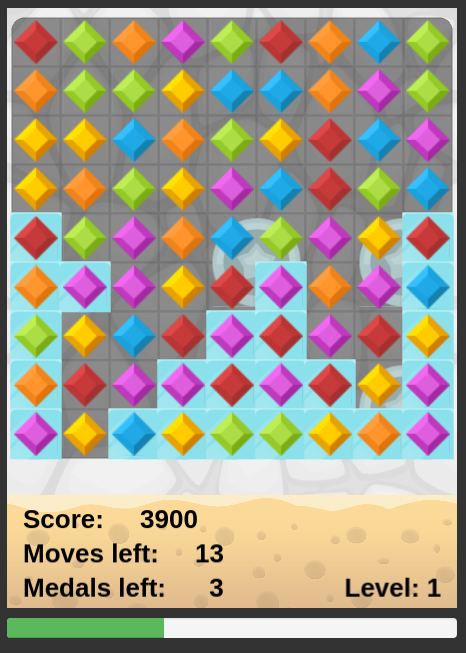
\includegraphics[width=0.4\textwidth]{media/img/screen3Medals}
	\caption{Gem Island: a match three game.}\label{f:gameMedals}
\end{figure}


The game of Gem Island is not more challenging for AI than Go, however, the stochastic nature of the game leads to a comparable search space and a much larger branching factor. For example, the branching factor for Go is 200 on average \cite{Gelly2012} while for match three it is conservatively 1080. This branching factor can also reach a value of up to $1 \times 10^{60}$ as it is theoretically possible to reach any state from one move.

We then create an AI program that successfully beats match three with a win rate of 85\% and mean of 13 moves to finish (out of 20). This AI uses several variants of Monte Carlo Tree Search (MCTS) including no evaluation function, a crude evaluation function, and a neural network based function. The main contribution of this report is the comparison of MCTS with varying evaluation functions and we find that the MCTS with a crude evaluation function performs best. The second major contribution is the game of match three itself, which has an open source application programming interface (API) tailored for AI research including gathering training data, easy access to the game state, and simple method of connecting AI controllers.

\chapter{Literature Review}
In this chapter we highlight the literature required to complete and understand this thesis.
\section{The Agent}
In this dissertation we refer to the AI program as the Agent. Where the agent senses the environment, makes some rational decision, then acts upon the environment. The environment in this case is the match three game; Gem Island.

An agent is anything that perceives the environment through sensors and acts upon it through actuators \cite{Russell2016}. A rational agent is an agent which chooses the best action value given some reward function. In other words, it makes the right decision given some state of the environment. For example, if we have a self-driving car and it sees a person on the road through some camera sensors, the right decision would be to stop.

The agent program is how it maps the state to an action and it is this which makes the agent rational. A optimum agent program would be perfectly rational whereas a suboptimal program would select actions at random.

\section{Decision Theory}
Decision theory is the theory of making the best decisions based upon utility and probability theory. Where utility is the `usefulness' of a state or, in other words, the happiness of the agent in a certain state. Utility is agent specific as for example two agents in chess, one white and the other black, the white agent would prefer a state where it won much more than the black agent. 



\section{Markov Decision Process}\label{s:mdp}
Markov Decision Processes (MDPs) are a way of modelling a sequence of decisions where there are some probabilistic and deterministic elements. The four components used to model an MDP are \cite{Russell2016}:

\begin{itemize}
	\item $S$: A set of states, with $s_0$ being the initial state.
	\item $A$: A set of actions.
	\item $T(s,a,s')$: A transition model that determines the probability of reaching state $s'$ if action $a$ is applied to state $s$.
	\item $R(s)$: A reward function.
\end{itemize}
For any given state $s$, you have a set of legal action $a \in A$, and there is some probability  you move to a new state $s'$ by the Equation:
\begin{equation}\label{mdp}
P(s' | s,a)
\end{equation}
Markov Decision Processes satisfy the Markov property which means transitioning to state $s'$ is only dependent on its immediate previous state $s$, but independent of all other states. For every transition you receive a reward $R(s)$, according to the state and the overall goal of MDPs is to find an optimal policy (action sequence) to maximise the sum of all the rewards from each state.


\section{Partially Observable Markov Decision Process}\label{s:pomdb}
Words.
\section{Game Theory}
Game theory extends decision and is concerned with how multiple self-interested agents interact. (What does self-interested mean). Single player with stochastic elements can be modelled using game theory as the agent playing against the `puzzle maker,' where the puzzle maker is, for example, the dealer in blackjack.

A game is generally represented with the following terms \cite{Browne2012}:

\begin{itemize}
	\item $S$: A set of states, with $s_0$ being the initial state.
	\item $S_T \subseteq S$: The set of terminal states.
	\item $n \in N$: The number of players.
	\item $A$: A set of actions.
	\item $T(s,a,s')$: A transition model that determines the probability of reaching state $s'$ if action $a$ is applied to state $s$.
	\item $R(s)$: A reward function.
\end{itemize}



\section{Monte Carlo Tree Search}\label{s:mcts}
Monte Carlo Tree Search (MCTS) has been ground-breaking in helping solve games with intractable search space. Previous brute force approaches could not handle the search space of Go as it could not fit into memory or it would take too long to compute. MCTS overcomes this by simulating games and recording the outcome $W$, i.e. win or lose. This process is repeated hundreds or thousands of times to record the outcome and number of plays for each move and its previous state (state-action pairs). After $N$ simulations the move with the best win rate (denoted as $Z(s,a)$) is selected which is given by:

\begin{equation}\label{utility}
Z(s,a) = \frac{W}{N}
\end{equation} 

Where $s$ is the state and $a$ is the action taken from state $s$, $W$ is the win count, and $N$ is the number of times action $a$ has been selected from state $s$.

Monte Carlo Tree Search builds a tree data structure in memory representing sequences of actions and each nodes stores the win rate ($W$ and $N$). This building process can be broken into four phases; selection, expansion, roll-out and back-propagation.

To begin with we take the current state of the game as the root node (State $s_0$) of the tree as shown in Figure \ref{f:initTree}.
\begin{figure}
	
	\caption{Initial tree}\label{f:initTree}
\end{figure}
We then simulate a game for each legal action of that root node. This means we now have statistics for each action and its subsequent state. Figure \ref{f:initSim} shows the state $s_0$ as the root node, the legal actions as its branches, and the subsequent states of the actions as children nodes.
\begin{figure}
	
	\caption{Initial Sims}\label{f:initSim}
\end{figure}
After initialising the tree we can enter the selection phase. This involves using an algorithm (refer Subsection \ref{s:tPolicy}) to pick the `best' child node as per the algorithm. This process is repeated with subsequent child nodes until we reach one without any statistics. Selecting these nodes presents a problem of exploiting actions with known good win rates and exploring alternative actions which might have better win rates. This problem is known as the multi-armed bandit problem which has been studied extensively in literature and is discussed further in Section \ref{s:tPolicy}.

Reaching a node with no statistics means we enter the expansion phase. The new node is added to the tree and is initialised with the statistics $N=0$ and $W=0$. Following on from the example shown in Figure \ref{f:initSim}, the expansion phase is illustrated in Figure \ref{f:treeExpansion}.
\begin{figure}
	
	\caption{Tree expansion}\label{f:treeExpansion}
\end{figure}
From there we enter the roll-out phase which means rapidly simulating the remaining moves of the game with a simple default policy (refer Subsection \ref{s:rollOut}) as depicted in Figure \ref{f:treeRollout}.
\begin{figure}
	
	\caption{Tree Rollout}\label{f:treeRollout}
\end{figure} 
Once we reach the end of the game (terminal state), we can determine if we win or lose. As the name of the final phase suggest, this outcome is back-propagated up the sequence of moves carried out in the tree. For example, if the outcome was a win each node in this sequence would have its win and play count increased by one. This process is illustrated in Figure \ref{f:treeBackprop}, note that we do not have any expanded nodes in the roll-out phase so no statistics are recorded in that section.

\begin{figure}
	
	\caption{Tree Backprop}\label{f:treeBackprop}
\end{figure}

\subsection{Tree Policy}\label{s:tPolicy}
The multi-armed problem is a problem of a gambler maximising his cumulative reward from several slot machine (one-armed bandits). The gambler plays a slot machine to get a reward from some unknown probability distribution, the more he gambler plays, the more accurate he can estimate the distribution and therefore the expected (read average) reward. The gambler must decide which machine to play, how many times to play it, and when to switch to another. He must balance this in order to maximise his cumulative reward over all the slot machines played. 

The multi-armed bandit problem is a way of modelling the selection process of a child node in a Monte Carlo tree. Many solution exist but the most common and successful one is the Upper Confidence Bound for Tree (UCT) \cite{Browne2012}. This uses the formula:

\begin{equation}\label{e:UCT}
Z(s,a) = \frac{W(s,a)}{N(s,a)} + C\sqrt{\frac{\log(N(s))}{N(s,a)}}
\end{equation} 


Where $N(s,a)$ is the number of times action $a$ has been selection from state $s$, $W(s,a)$ the number of times this action has resulted in a win at the terminal state, $N(s)$ is the total number of simulations played from state $s$, and $C$ is a tuning constant.

UCT is used to calculate the value of the child nodes and the one with the highest value is selected. This is repeated to follow a sequence through the current tree until we come to a node which has not been explored before. UCT comprises two main components; the exploitation factor $\frac{W(s,a)}{N(s,a)}$ representing the win rate, the exploration factor $\sqrt{\frac{\log(N(s))}{N(s,a)}}$ representing how many times a node has been selected, and $C$ which is tuned to how much the exploration factor should have an impact. The exploitation factor is high for successful nodes and the exploration factor is high for nodes that have been explored very few times. This means the UCT tree policy favours actions that result in a good win rate but will still select actions if they have not been explored very many times.

There are many other bandit-based algorithms to potentially improve upon the tree policy. Alternative upper confidence bound algorithms include UCB1-Tuned \cite{Auer2002}, Bayesian UCT \cite{Grunwald2010}, and EXP3 \cite{Auer1995} \cite{Audibert2009}, however the policy is not the focus of this report is therefore not covered extensively. The papers for the alternative algorithms mentioned above are included in the references for the reader to view at his leisure.

\subsection{Roll-out}\label{s:rollOut}
The roll-out phase is designed for rapid play-out to reduce the overall computational expense of Monte Carlo Tree Search. This is achieved by having a default policy which can be as simple as always selecting the move location at position (0,0) in subsequent states until a terminal state is reached. A more common approach is sampling over a uniform random distribution of legal moves but they can also be tailored to suit the problem domain to dramatically improve performance \cite{Browne2012}.
\subsection{One Look-ahead}
\subsection{One Look-ahead with Roll-out}
\subsection{Full Monte Carlo Tree Search}
\section{Neural Networks and Deep Learning}
In this section we cover the background literature on neural network layers, convolutional networks, and deep learning.

\subsection{Neural Networks}
A neural network is a style of programming where programs learn from observing data. It can be thought of as a function which must first be taught how to do something so that it can give accurate answers. They are commonly used in state-of-the-art programs for image recognigtion, speech recognition, and natural language procession. In other words, they are excellent at classification and identifying patterns in complex data.

Neural networks are made up of an input, output, and one hidden layer as shown in Figure \ref{f:NN}.
\begin{figure}
	
	\caption{Neural network}\label{f:NN}
\end{figure}
Whereas deep neural networks are the same except with more than one hidden layer.

\subsection{Training Neural Networks}

\subsection{Convolution Layer}
In this subsection we describe the convolution operation, how it is used in the convolutional layer, and what advantages they have.

A convolution is essentially a weighted average. It can be used to detect edges in an image or create blur effects, it all depends on the weights in the convolution. Imagine we have a very small three by three image as shown in Equation \ref{e:smallImage}, where each number is a pixel and the value represents a colour. Also shown is a filter which is typically much smaller and in our image is shown as a two by two matrix.

We then compute the first convolution by placing the filter over the four top left numbers in the image which results in the operation shown in Equation \ref{e:convOp} resulting in a single value. This is repeated repeated 3 more times by sliding the filter across the image to get four values in toal as shown in Equation \ref{e:convOp2}.

\begin{equation}\label{e:smallImage}
image = 
\left[ \begin{array}{ccc}
0 & 1 & 3 \\
2 & 1 & 4 \\
1 & 5 & 6 \\
\end{array}\right]
filter = 
\left[\begin{array}{cc}
1 & 2 \\
3 & 4 \\
\end{array}\right]
\end{equation}

\begin{equation}\label{e:convOp}
\left[\begin{array}{ccc}
0 \times 1 & 1 \times 2 & 3 \\
2 \times3 & 1 \times 4 & 4 \\
1 & 5 & 6 \\
\end{array}\right]
\Rightarrow
cell(0,0) = (1+2+6+4)/4 = 3
\end{equation}

\begin{equation}\label{e:convOp2}
Convolved Image=
\left[\begin{array}{cc}
3 & 5.5 \\
6.75 & 12 \\
\end{array}\right]
\end{equation}

The filter can have certain weights to detect edges, dark regions, and other attributes. If we now imagine a convolutional neural network we get something like the example illustrated in Figure \ref{f:CNNInput}. We repeat the previously described process on the input layer to produce the first hidden layer. The weights, depicted as lines in the illustration, are learnt by the neural network and shared for all neurons in the first hidden layer. One shared filter is called a feature map and allows you detect certain aspects of an image such as all vertical edges in the image. For each different aspect of an image you need another feature map and therefore convolutional neural networks are generally made up of several feature mappings. Figure \ref{f:CNN3Feature} shows three feature maps from the input layer to produce three different layers (channels) in the first hidden layer (3 channels of 24 by 24 neurons). Each layer would be detecting a different aspect of the image such as vertical, horizontal, and circular edges.

An advantage of a convolutional layer is that it takes into account the spatial structure of an image. This means it knows the top-left cell is next to the second top-left cell whereas in normal neural networks these two cells would be considered the same distance from each other as the top-left and bottom-right i.e. there is no distance metric.

Another advantage is the sharing of weights for each filter map. This greatly reduces the number of parameters to learn therefore significantly reducing the time to train a network. Before incorporating convolutional layers it was considered to hard to train image classifiers as they contain too much data.

\begin{figure}
	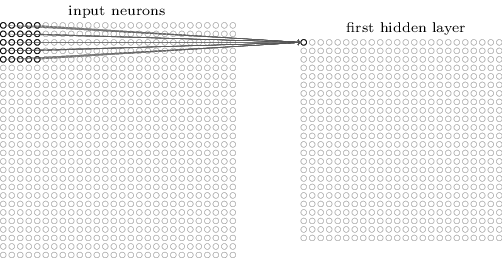
\includegraphics[width=\textwidth]{media/img/cnnInputAndHidden}
	\caption{Input and First Hidden Layer of a convolutional neural network \cite{Neilsen2015}}\label{f:CNNInput}
\end{figure}

\begin{figure}
	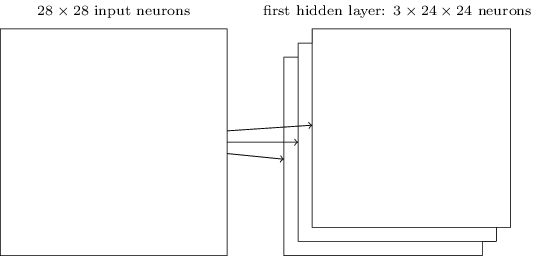
\includegraphics[width=\textwidth]{media/img/cnn3FeatureMaps}
	\caption{Three feature maps from the input layer \cite{Neilsen2015}}\label{f:CNN3Feature}
\end{figure}


\subsection{Max Pooling Layer}
Max pooling is typical pooling layer that occurs immediately after convolution layers. This layer is similar to a convolutional layer except the filter selects the maximum value rather than computing the weighted average. For example, if we have the same image as shown in Equation \ref{e:smallImage} and apply a two by two max-pooling filter to the four top left numbers we get a value of two as it is the maximum. This is repeated three more times to get the hidden layer as shown in Equation \ref{e:maxPool}.

\begin{equation}\label{e:maxPool}
maxPooledImage=
\left[\begin{array}{cc}
2 & 4 \\
5 & 6 \\
\end{array}\right]
\end{equation}

The advantage of this to reduce the number of parameters by even more without any significant loss in data quality.
\subsection{Dropout Layer}




\chapter{Problem Domain}\label{ch:pb}
In this chapter we classify the game of match three in terms of determinism, hidden information, number of players.

The game of Gem Island (refer Section \ref{s:gamed}) is classified as non-deterministic due to its stochastic nature and hidden information. The non-deterministic elements are:
\begin{itemize}
	\item Gem generation
	\item Hidden medals
\end{itemize}

Gems are created by randomly selecting a type between and including the range of 1 and 6. Medals are randomly placed underneath ice with the constraint that they do not overlap.

Gem Island is a single player game but can be modelled as a two player zero sum game with the player playing against the stochastic elements (commonly referred to as the puzzle maker). The player must win (1) and puzzle maker lose (-1), or vice versa, so the outcome sums to zero. Visualising the game like this helps with modelling it as a Monte Carlo Tree (refer Chapter \ref{s:mcts})

Gem Island involves making a sequence of decisions to win or lose the game and it has hidden information therefore it can be classified as a Partially Observable Markov Decision Process (refer Sections \ref{s:mdp} and \ref{s:pomdb}).

For example in Gem Island, if you match three gems of the same type, the matched gems will disappear, existing ones will fall leaving empty cells at the top where three gems will randomly appear. As there are 6 gem types, this means we have $6^3 = 216$ new states. This is the minimum number of new states from any move. It is also not uncommon for an entire row to be removed (9 gems) from a cross bonus (ref game rules) which results in $6^9=10,077,696$ new states. Each state has equal probability of occurring and is therefore non-deterministic.



\chapter{Solution Design}
In this chapter we discuss how to solve the non-deterministic game of Gem Island by applying current literature of Monte Carlo Tree Search (MCTS) and neural networks (refer Chapter \ref{ch:pb} for problem domain). Moreover, we introduce a number of MCTS designs each with a different evaluation function, which are:

\begin{itemize}
	\item No evaluation function
	\item Crude evaluation function
	\item Heuristic based evaluation function
	\item Evaluation network with outcome labels
	\item Evaluation network with utility labels
\end{itemize}

\section{Monte Carlo Tree Search}
In this section we outline the design of the modified selection and expansion process, the `opponent' modelling to account for the stochastic medal placements, and the roll-out and back-propagation phases.

Monte Carlo Tree Search works well in deterministic games because a tree can be built to store the win rate of state-action pairs (cite). Building a tree is also useful for some non-deterministic games where the number of possible states from the previous state (branching factor) is relatively low. However, in Gem Island the branching factor is at minimum 216 (three gems) and can easily reach 10,000,000 (9 gems). In addition, the possible medal locations under the ice contribute to this branching factor. Furthermore, there is equal chance of reaching any one of those 10 million states. This means if we store a sequential state we have a very low likelihood of getting the same state in a following simulation ($1 \times 10^{-5}\%)$. If we store a following sequence (level 2 in the tree) this chance drops significantly to $1 \times 10^{-10}\%$. Because of this very low chance of reaching the same state we do not expand the tree at all in our MCTS design. Rather we only store the legal actions from the root state and their corresponding win and play counts. This means we use the roll-out phase with the default policy (refer Section \ref{s:rollOut}) for the remaining moves. This design is referred to as Flat UCT in literature (cite). A benefit of this is efficient memory storage as only one level of actions is stored and the encoded state (refer Section \ref{s:state}) representations are ignored. Furthermore, this reduces the back-propagation process from iterating over all expanded nodes in the sequence to simply adding the win and play count directly to the first action.



\section{No Evaluation Function}
The first design is a full Monte Carlo Tree Search without an evaluation function. This means the roll-out phase is played until the a terminal state and the action selected from the root state has its win and play count updated.

\section{Crude Evaluation Function}
This design incorporates a crude evaluation function which gives a state a rating in the range of zero to one, where one represents a certain win. This also means the roll-out phase can go to any depth, such as one look-ahead or fives moves. The function is considered crude as its only feature is to count the portion of medals remaining. The portions count is normalised by dividing it by the total portions remaining in the root state. This feature was chosen as removing all the medals is the goal of the game and is therefore the most important feature.

\section{Heuristic Based Evaluation Function}
The heuristic based evaluation function is similar to the crude version except it includes additional features. These features are designed to encourage exploration under the ice, remove as many gems as possible, and to finish the game quickly. In doing so we hope to increase the overall win rate of the AI.
\section{Evaluation Network with Outcome Labels}
The Evaluation network with outcome labels is a simple neural network with a convolutional layer with 6 feature mappings and a 50\% drop-out layer. The architecture of this network is illustrated in Figure \ref{f:nnArch}.

\begin{figure}
	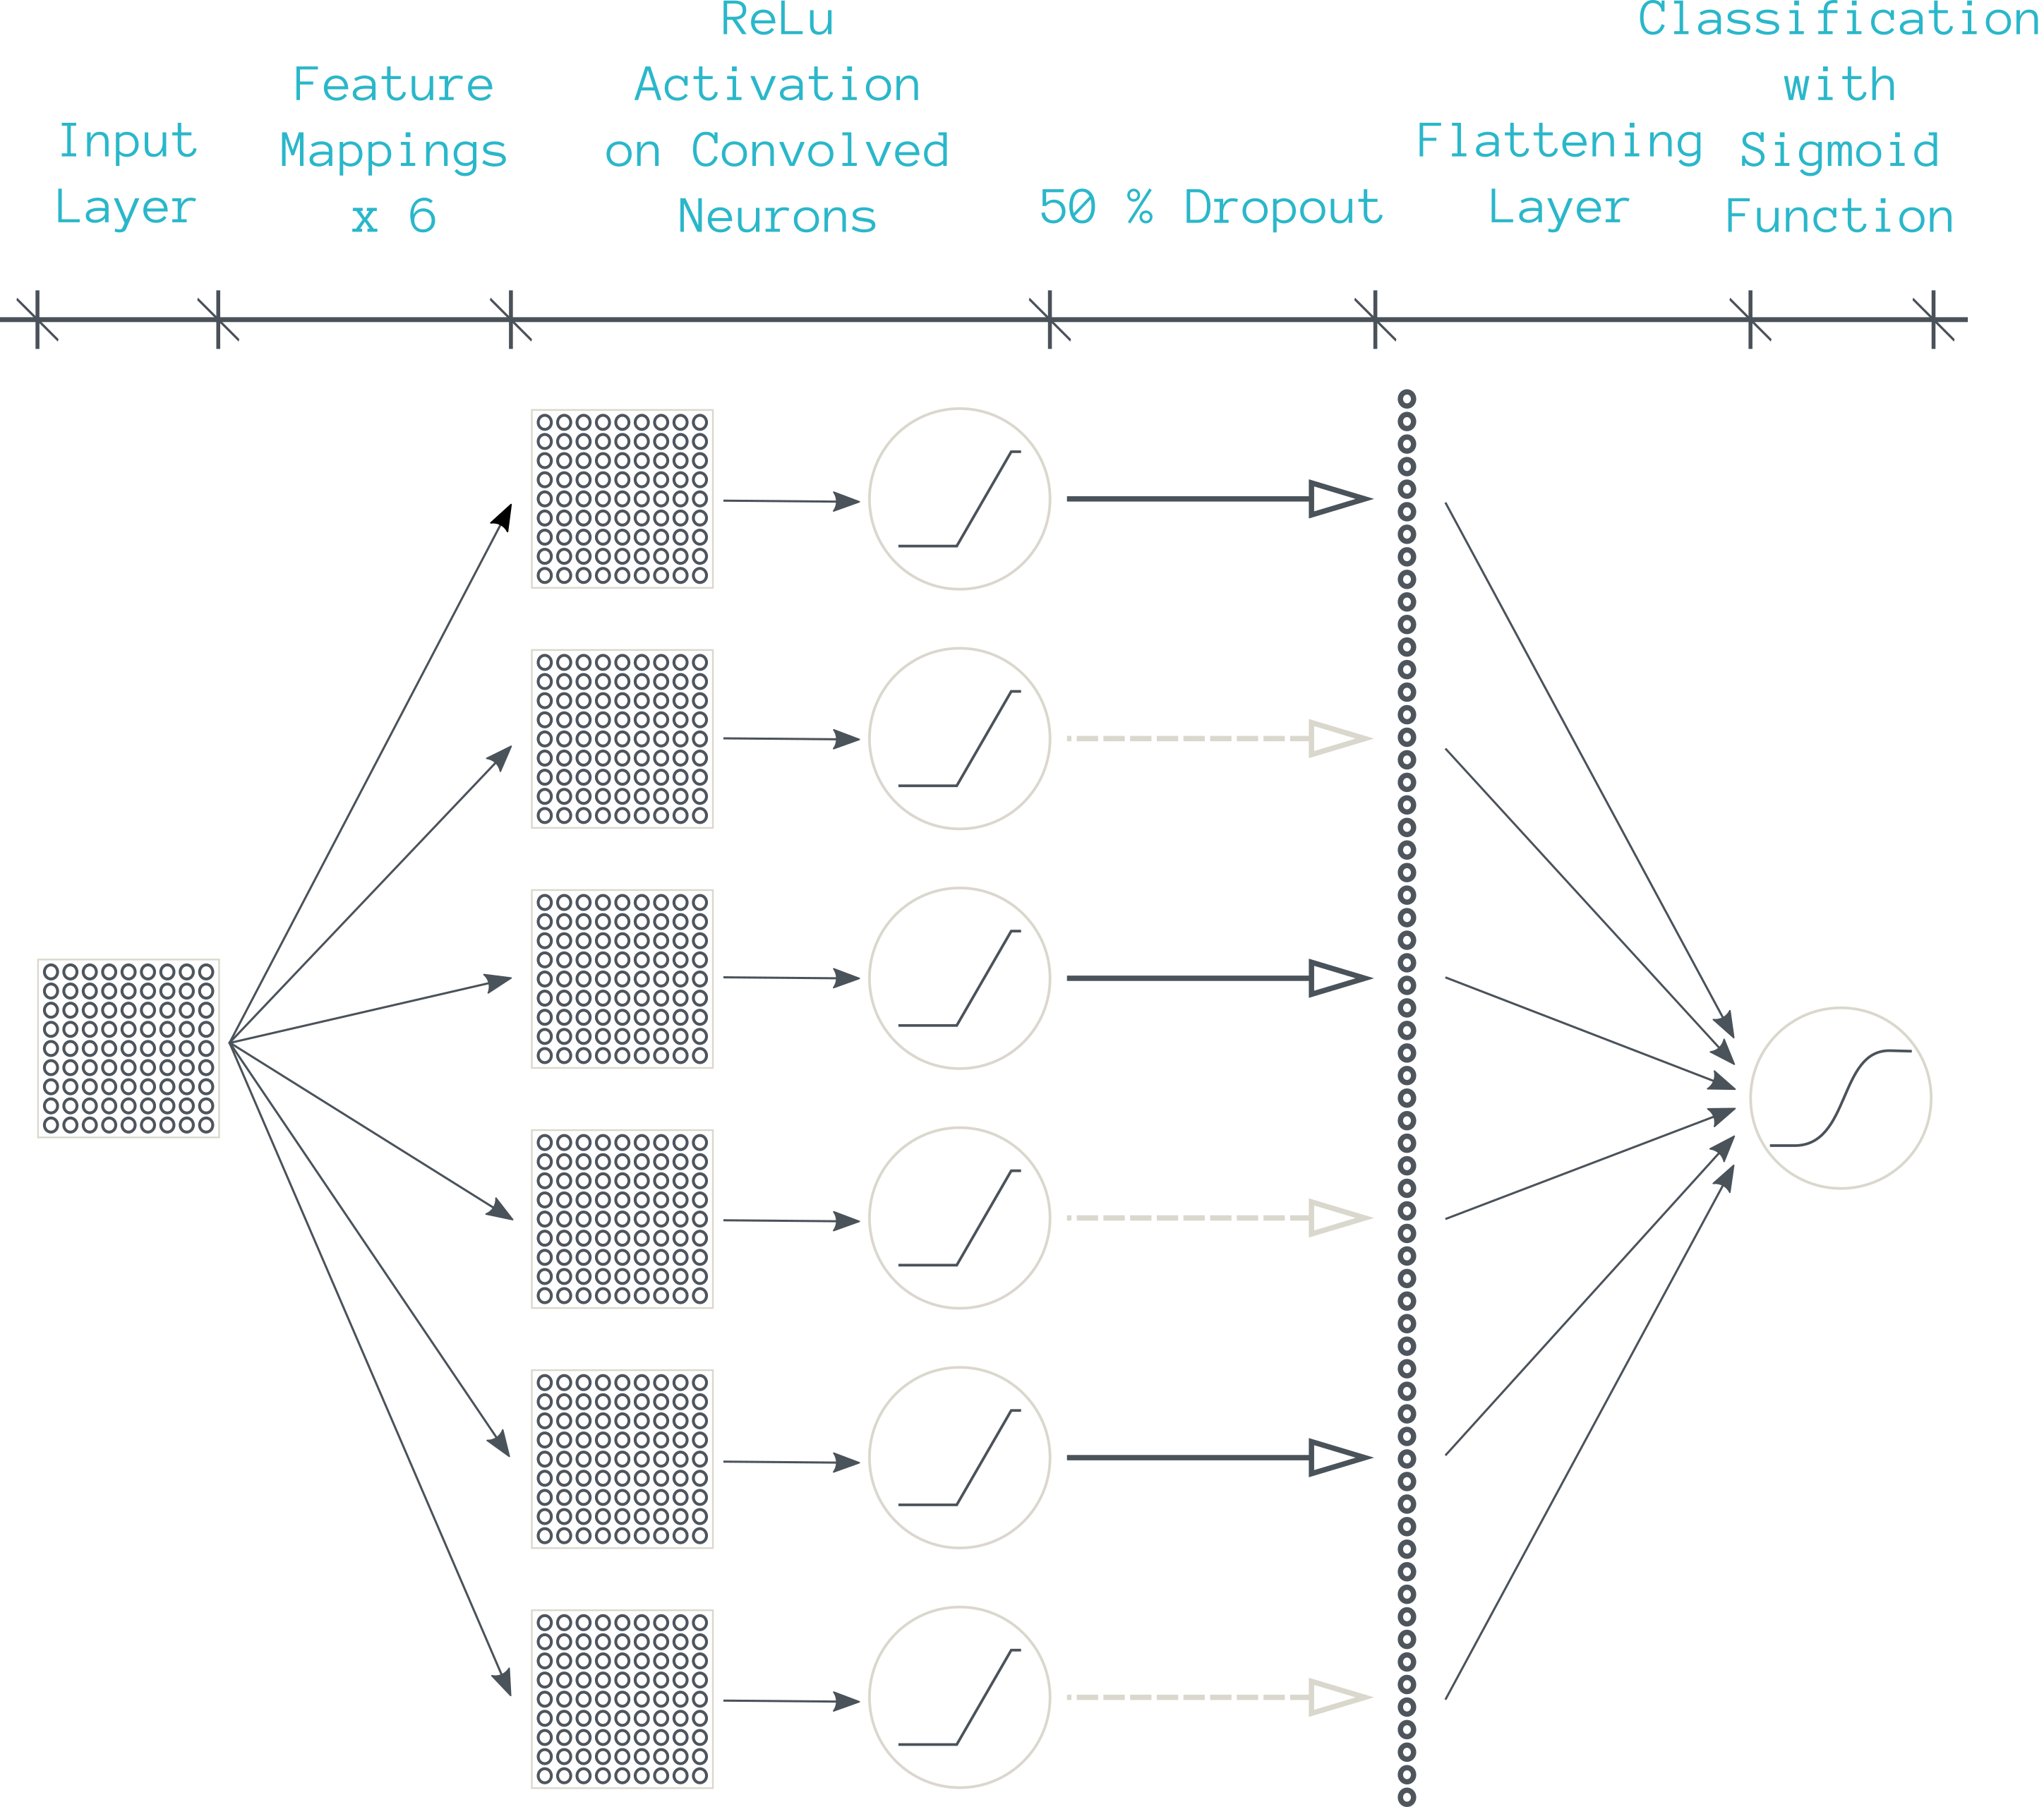
\includegraphics[width=\textwidth]{media/img/nnArch}
	\caption{The architecture of the evaluation network trained with outcome labels.}\label{f:nnArch}
\end{figure}
 The network was trained by selecting one state (refer Section \ref{s:state}) at random from each of the six thousand games that were recorded from the website (refer Section \ref{s:website}). Only one state was selected from each game to avoid having correlated states. The states were changed into fourteen one-hot encoded states to make training the network simpler. This means the six gem types are now split into by six different layers where the first layer is a $9 \times 9$ array composed of ones if a type one gem existed at that position and zero if not. The next three layers represent the bonus types, one layer for ice, and four layers for medal portions. An interpretation of how this would look is illustrated in Figure \ref{f:nnTraining}.
 
 \begin{figure}
 	\centering
 	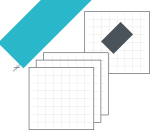
\includegraphics[width=0.5\textwidth]{media/img/nnTraining}
 	\caption{The one-hot encoded states for training the neural networks.}\label{f:nnTraining}
 \end{figure}
 
For each state we have the outcome of that game which is what was used as the training labels. This means if state $s_n$ belonged to a game which resulted in a win it would be assigned a label of one and zero if it was a loss. These corresponding labels were stored in a one-dimensional array as shown in Figure \ref{f:nnLabels}.

 \begin{figure}
	\centering
	
\includegraphics[width=0.13\textwidth]{media/img/nnLabels}
	\caption{The corresponding labels for the training data.}\label{f:nnLabels}
\end{figure}

There is also a risk of over-fitting to the gem types rather than the pattern of gems. To avoid this we permuted the states to get every every combination and to make it gem type agnostic. Consequently this increased our training data by a factor of 720.

\section{Evaluation Network with Utility Labels}
This network used a similar design to make it comparable to the outcome label network, however, instead it used what we named utility labels. These labels were computed by running Monte Carlo Tree Search on each state and selecting the maximum action win rate. In other words it works out the likelihood of winning from an arbitrary state.

\chapter{Technical Requirements}
To build an agent to win match three we also needed an open source version of the game so we could get the game state and control it with AI. Therefore we designed and implemented our own version which is outlined in Section \ref{s:gamed}. 

To train the neural network we needed data. To gather this data we built a website that recorded users moves and logged it all in files on the server. The design of the website is outlined in Section \ref{s:website}.

\section{Game Design: Gem Island}\label{s:gamed}

\begin{figure}
	\centering
	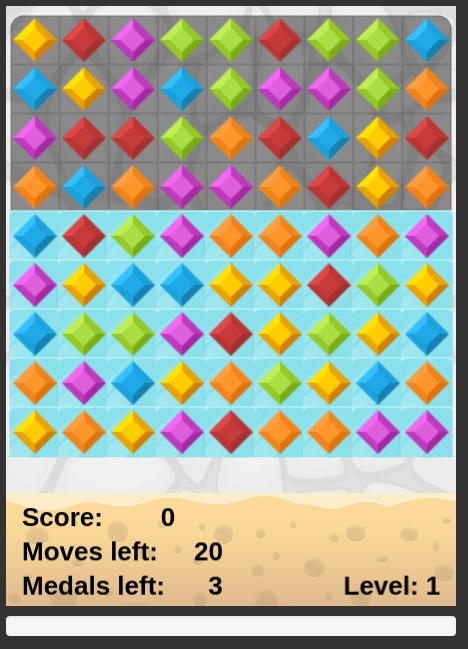
\includegraphics[width=0.4\textwidth]{media/img/screen2}
	\caption{Gem Island.}\label{f:gemIslandGame}
\end{figure}

\section{State Representation}\label{s:state}
The AI program must be able to read the current state of the game. This means the arrangement of the gems, ice, and medals must all be encoded so the program can determine what is shown on screen. For this we chose a simple string representation where a sequence of four numbers represented one cell in the $9 \times 9$ grid. The four numbers represented the gem type (colour), the bonus type, if ice was present, and a medal portion if it existed. This sequence of four numbers was repeated 81 times to represent each cell in the grid. The AI program could then decode this state string and simulate games via the Monte Carlo Search Tree.

\section{Website Design}\label{s:website}


\chapter{Artificial Intelligence Performance Analysis}
\section{Analysis Methodology}
\section{Results}
Results from analysis. \cite{Browne2012}
Which algorithms and parameters performed better.
Why did they perform better.
Why did some fail.
\section{Comparison of Evaluation Functions}
How the analysis was performed (how to reproduce results).


\chapter{Evaluation of Project}
In this chapter we discuss the limitation of the author and evaluate the difficulty and usefulness of the project.

\chapter{Conclusion}
Summary of results and findings. Recommendations of design and parameters for similar AI and game design.

\chapter{Further Study}
In this chapter we discuss possible future studies using the findings in this report and also the existing game API.



\backmatter
\chapter{References}
\printbibliography[heading=none]
%\bibliographystyle{plain}
%\bibliography{bibeg}

\chapter{Appendices}
\end{document}